\documentclass[aspectratio=169, 11pt]{beamer}
\usepackage{fontspec}
\usepackage{amsmath, amssymb}
\usepackage{graphicx}
\usepackage{booktabs}
\usepackage{tikz}
\usepackage{xcolor}

\setmainfont{Noto Sans CJK KR}
\setsansfont{Noto Sans CJK KR}
\linespread{1.15}

\usetheme{Madrid}
\usecolortheme{seahorse}
\setbeamertemplate{navigation symbols}{}
\setbeamerfont{frametitle}{size=\large, series=\bfseries}
\setbeamerfont{title}{size=\Large, series=\bfseries}

\title[Bayesian Multilevel Model]{베이지안 다층모형(Bayesian Multilevel Model)\\왜, 어떻게, 무엇이 좋은가}
\subtitle{Gelman, Hill \& Yajima (2012) 와 주월랑(2023) 사례를 중심으로}
\author{재분석 강의자료}
\institute{}
\date{}

\begin{document}

%---------- Slide 1: Title ----------
\begin{frame}
\titlepage
\end{frame}

%---------- Slide 2: Outline ----------
\begin{frame}{학습 목표}
\begin{itemize}
\item 빈도주의 검정(t-test, ANOVA)의 \textbf{한계} 이해
\item 다중비교(multiple comparisons) 문제와 Bonferroni 보정의 \textbf{대가}
\item 베이지안 다층모형의 \textbf{기본 아이디어}: ``효과들이 정규분포를 따른다''
\item t-test와 ANOVA가 다층모형의 \textbf{특수 경우}임을 이해
\item 부분 풀링(partial pooling)의 직관과 \textbf{Type M 오류} 완화
\item Python(numpyro) 으로 \textbf{10줄 안에} 다층모형 적합하기
\end{itemize}
\end{frame}

%---------- Slide 3: Motivation - Coin Example ----------
\begin{frame}{도입 — 동전 두 개 이야기}
두 친구가 각자 동전을 던졌습니다.
\vspace{0.4cm}
\begin{columns}
\column{0.5\textwidth}
\begin{block}{친구 A}
\begin{itemize}
\item 동전을 \textbf{10번} 던졌다
\item 그 중 \textbf{9번} 앞면
\item $\hat p = 0.9$
\item 양측 $p$값 $\approx 0.022$ $<$ 0.05 \textbf{유의}
\end{itemize}
\end{block}
\column{0.5\textwidth}
\begin{block}{친구 B}
\begin{itemize}
\item 동전을 \textbf{1000번} 던졌다
\item 그 중 \textbf{540번} 앞면
\item $\hat p = 0.54$
\item 양측 $p$값 $\approx 0.011$ $<$ 0.05 \textbf{유의}
\end{itemize}
\end{block}
\end{columns}
\vspace{0.4cm}
\centering
\large 둘 다 ``유의''이지만, 두 사람의 결론을 \emph{똑같이} 믿어야 할까?
\end{frame}

%---------- Slide 4: Type M Error ----------
\begin{frame}{Type M 오류 — 효과 크기의 과장}
\textbf{만약 진짜 동전이 약간만 편향($p_{\text{true}} = 0.55$)이라면?}
\vspace{0.3cm}

\begin{tabular}{lcc}
\toprule
 & 친구 A (9/10) & 친구 B (540/1000) \\
\midrule
참 편향 $|p-0.5|$ & 0.05 & 0.05 \\
추정 편향 $|\hat p-0.5|$ & \textbf{0.40} & 0.04 \\
\textbf{과장 비율} & \textbf{8 배} & 0.8 배 \\
95\% 신뢰구간 & $[0.71, 1.00]$ (매우 넓음) & $[0.51, 0.57]$ (좁고 신뢰) \\
\bottomrule
\end{tabular}

\vspace{0.4cm}
\begin{itemize}
\item 친구 A의 ``유의'' 결과는 \textbf{Type M 오류(magnitude error)}의 전형
\item 검정력 부족(underpowered) 연구에서 ``유의''로 나온 결과는 효과 크기를 \textbf{체계적으로 과장}
\item Gelman \& Carlin (2014): ``승자의 저주(winner's curse)''
\end{itemize}
\end{frame}

%---------- Slide 5: Multiple Comparisons ----------
\begin{frame}{다중비교 문제 — 검정을 많이 하면?}
유의수준 $\alpha = 0.05$로 \textbf{독립적} 검정 $k$개를 수행한다고 하자.

\vspace{0.3cm}
적어도 하나가 ``유의''로 잘못 판정될 확률(가족별 오류율, FWER):
$$
\text{FWER} = 1 - (1 - \alpha)^k
$$

\vspace{0.3cm}
\begin{tabular}{ccc}
\toprule
$k$ (검정 수) & FWER & 의미 \\
\midrule
1 & 5\% & 정상 \\
5 & 23\% & 우려 \\
8 & 34\% & 심각 \\
20 & 64\% & 매우 심각 \\
38 (주월랑) & 86\% & 거의 확실히 거짓 양성 \\
\bottomrule
\end{tabular}

\vspace{0.3cm}
\centering
\textbf{검정을 많이 할수록 ``우연한 유의''가 보장된다.}
\end{frame}

%---------- Slide 6: Bonferroni ----------
\begin{frame}{고전적 해결책 — Bonferroni 보정}
임계값을 $\alpha/k$로 낮춘다 (즉 더 보수적으로 판단).
\vspace{0.3cm}

\begin{block}{문제}
\begin{itemize}
\item 1종 오류는 줄어들지만 \textbf{2종 오류(검정력 손실)}가 커짐
\item 진짜 효과도 ``비유의''로 놓쳐버림
\item 사회과학에서 ``효과가 정확히 0''이라는 귀무가설이 \textbf{비현실적}
\end{itemize}
\end{block}

\vspace{0.3cm}
Gelman의 핵심 주장:
\begin{quote}
\centering
\itshape ``We don't (usually) have to worry about multiple comparisons.''\\
$-$ Gelman, Hill \& Yajima (2012)
\end{quote}

근거: \textbf{다층모형(multilevel model)}이 다중비교 문제를 \emph{자동으로} 해결.
\end{frame}

%---------- Slide 7: Multilevel Model Basic ----------
\begin{frame}{다층모형의 기본 식 — 단 한 줄}
\large
$$
y_i = \mu + \alpha_{\text{group}[i]} + \varepsilon_i
$$
$$
\alpha_g \sim \mathcal{N}(0, \sigma_\alpha^2), \quad \varepsilon_i \sim \mathcal{N}(0, \sigma_y^2)
$$

\normalsize
\vspace{0.3cm}
\textbf{해석:}
\begin{itemize}
\item $\mu$: 전체 평균(grand mean)
\item $\alpha_g$: 그룹 $g$의 효과(전체평균에서 벗어난 편차)
\item ``그룹 효과들이 정규분포를 따른다''는 가정 — 핵심!
\item $\sigma_\alpha$: 그룹들 사이의 변동 정도 (데이터로부터 추정)
\item $\sigma_y$: 그룹 내 개인차
\end{itemize}

\vspace{0.3cm}
\centering
\textbf{이 단순한 식 하나가 t-test, ANOVA, 사후비교를 모두 포괄한다.}
\end{frame}

%---------- Slide 8: Three Pooling Regimes ----------
\begin{frame}{$\sigma_\alpha$ 가 결정하는 세 가지 체제(regime)}
\centering
\begin{tabular}{lll}
\toprule
$\sigma_\alpha$ 값 & 모형 행동 & 빈도주의 대응 \\
\midrule
0 (또는 매우 작음) & 완전 풀링(complete pooling) & 그룹 차이 무시 \\
& 모든 $\alpha_g = 0$ & ($H_0$ 채택) \\
\midrule
$\infty$ (또는 매우 큼) & 풀링 없음(no pooling) & 각 그룹 독립 추정 \\
& 각 $\alpha_g$ 독립 추정 & (전통적 t-test/ANOVA) \\
\midrule
\textbf{데이터로 추정} & \textbf{부분 풀링(partial pooling)} & \textbf{없음(베이지안 고유)} \\
& 작은 표본은 평균 쪽으로 끌어당김 & \\
\bottomrule
\end{tabular}

\vspace{0.4cm}
\textbf{핵심:} $\sigma_\alpha$를 \emph{데이터로부터 추정}한다는 점이 다층모형의 위력.
\end{frame}

%---------- Slide 9: t-test correspondence ----------
\begin{frame}{t-test 대응 — 수학적 다리}
\textbf{두 그룹 비교를 다층모형으로 표현:}
$$
y_i = \mu + \alpha_{g[i]} + \varepsilon_i, \quad g \in \{1, 2\}
$$

\vspace{0.2cm}
$\sigma_\alpha \to \infty$ 극한에서 사후분포:
$$
\alpha_1 - \alpha_2 \mid y \sim \mathcal{N}\!\left(\bar y_1 - \bar y_2,\ \sigma_y^2(1/n_1+1/n_2)\right)
$$

\vspace{0.2cm}
이 식은 \textbf{빈도주의 t-검정의 표본분포와 완전히 동일}.

\vspace{0.3cm}
\begin{tabular}{ll}
\toprule
빈도주의 t-검정 & 베이지안 다층모형 \\
\midrule
$t$ 통계량 & $\alpha_1 - \alpha_2$의 사후평균/사후 SD \\
양측 $p$값 & $2 \cdot \min P(\alpha_1 \gtrless \alpha_2 \mid y)$ \\
95\% 신뢰구간 (CI) & 95\% 신용구간 (credible interval) \\
\bottomrule
\end{tabular}
\end{frame}

%---------- Slide 10: ANOVA correspondence ----------
\begin{frame}{ANOVA 대응 — 같은 식, 더 많은 그룹}
\textbf{K개 그룹 비교:}
$$
y_i = \mu + \alpha_{g[i]} + \varepsilon_i, \quad g \in \{1, 2, \ldots, K\}
$$

\vspace{0.2cm}
빈도주의 ANOVA F-통계량 ${\approx}$ ``$\sigma_\alpha^2 / \sigma_y^2$가 얼마나 큰가''
$$
F \approx 1 + \frac{n \cdot \sigma_\alpha^2}{\sigma_y^2}
$$

\vspace{0.2cm}
\begin{tabular}{ll}
\toprule
빈도주의 ANOVA & 베이지안 다층모형 \\
\midrule
$F$ 통계량 & $\sigma_\alpha^2 / \sigma_y^2$의 사후분포 \\
$F$ 유의 & $\sigma_\alpha^2$ 의 95\% CI가 0 멀리 떨어짐 \\
사후비교(post-hoc, Tukey) & 모든 $\alpha_j - \alpha_k$ 의 공동 사후분포 \\
Bonferroni 보정 & \textbf{불필요} (부분 풀링이 자동 처리) \\
\bottomrule
\end{tabular}

\vspace{0.3cm}
\centering
\textbf{한 번 적합 → 모든 비교 동시 처리.}
\end{frame}

%---------- Slide 11: Case Study Setup ----------
\begin{frame}{사례연구: 주월랑(2023) 한국어 쓰기 태도 연구}
\textbf{연구 설계:}
\begin{itemize}
\item 외국인 유학생 $N = 86$
\item 21개 Likert 5점 정수 척도 문항 → 3개 하위범주
\begin{itemize}
\item 쓰기인식($P$, 문항 1$-$4)
\item 쓰기반응($R$, 문항 5$-$15)
\item 수행태도($A$, 문항 16$-$21)
\end{itemize}
\item Cronbach's $\alpha = 0.854$
\end{itemize}

\textbf{집단 표본 — 매우 불균형:}
\begin{tabular}{ll}
\toprule
요인 & 표본크기 \\
\midrule
학년 (5개 집단) & \textbf{54, 8, 9, 9, 6} \\
성별 (2개) & 27, 59 \\
TOPIK (5개) & 7, 14, 31, 23, 11 \\
어학원 (2개) & 69, 17 \\
\bottomrule
\end{tabular}
\end{frame}

%---------- Slide 12: Frequentist Analysis ----------
\begin{frame}{빈도주의 분석 — 주월랑의 방법}
주월랑은 4개 종속변수에 대해 각각:
\begin{itemize}
\item 학년 효과: \textbf{ANOVA} (5개 수준)
\item 성별 효과: \textbf{t-검정} (2개 수준)
\item TOPIK 효과: \textbf{ANOVA} (5개 수준)
\item 어학원 효과: \textbf{t-검정} (2개 수준)
\end{itemize}
$+$ Pearson 상관 22개 $\Rightarrow$ \textbf{총 약 38개 검정}, \emph{다중비교 보정 없음}.

\vspace{0.3cm}
유의하게 나온 결과는 \textbf{단 2개}:
\begin{tabular}{lll}
\toprule
검정 & 종속변수 & $p$값 \\
\midrule
ANOVA(학년) & 수행태도 & 0.026 \\
t-검정(성별) & 쓰기인식 & 0.007 \\
\bottomrule
\end{tabular}

\vspace{0.3cm}
\centering
\textbf{38번 던져 2번 ``유의''}. 우연일까, 실재일까?
\end{frame}

%---------- Slide 13: Bayesian Analysis ----------
\begin{frame}{베이지안 분석 결과 — 한 모형으로 모든 것}
\textbf{모형:}
$$
y_i = \mu + \alpha_{\text{year}[i]} + \beta_{\text{gender}[i]} + \gamma_{\text{topik}[i]} + \delta_{\text{inst}[i]} + \varepsilon_i
$$
$$
\alpha_j, \beta_g, \gamma_k, \delta_m \sim \mathcal{N}(0, \sigma_\cdot^2), \quad \sigma_\cdot \sim \text{HalfNormal}(1)
$$

\vspace{0.3cm}
\textbf{수행태도의 학년별 사후 차이 (가장 강하게 보이던 효과):}
\begin{tabular}{lcc}
\toprule
비교 & 사후 차이 (95\% CI) & 판정 \\
\midrule
2학년 $-$ 1학년 & $+0.371$ $[-0.011, +0.809]$ & 비유의 \\
3학년 $-$ 1학년 & $+0.227$ $[-0.088, +0.601]$ & 비유의 \\
4학년 $-$ 1학년 & $+0.303$ $[-0.021, +0.682]$ & 비유의 \\
EX $-$ 1학년 & $+0.028$ $[-0.370, +0.406]$ & 비유의 \\
\bottomrule
\end{tabular}

\vspace{0.3cm}
\centering
\textbf{빈도주의의 ``유의''가 베이지안에서는 모두 0을 포함.}
\end{frame}

%---------- Slide 14: Shrinkage ----------
\begin{frame}{부분 풀링 효과 — 수행태도 학년별 평균}
\centering
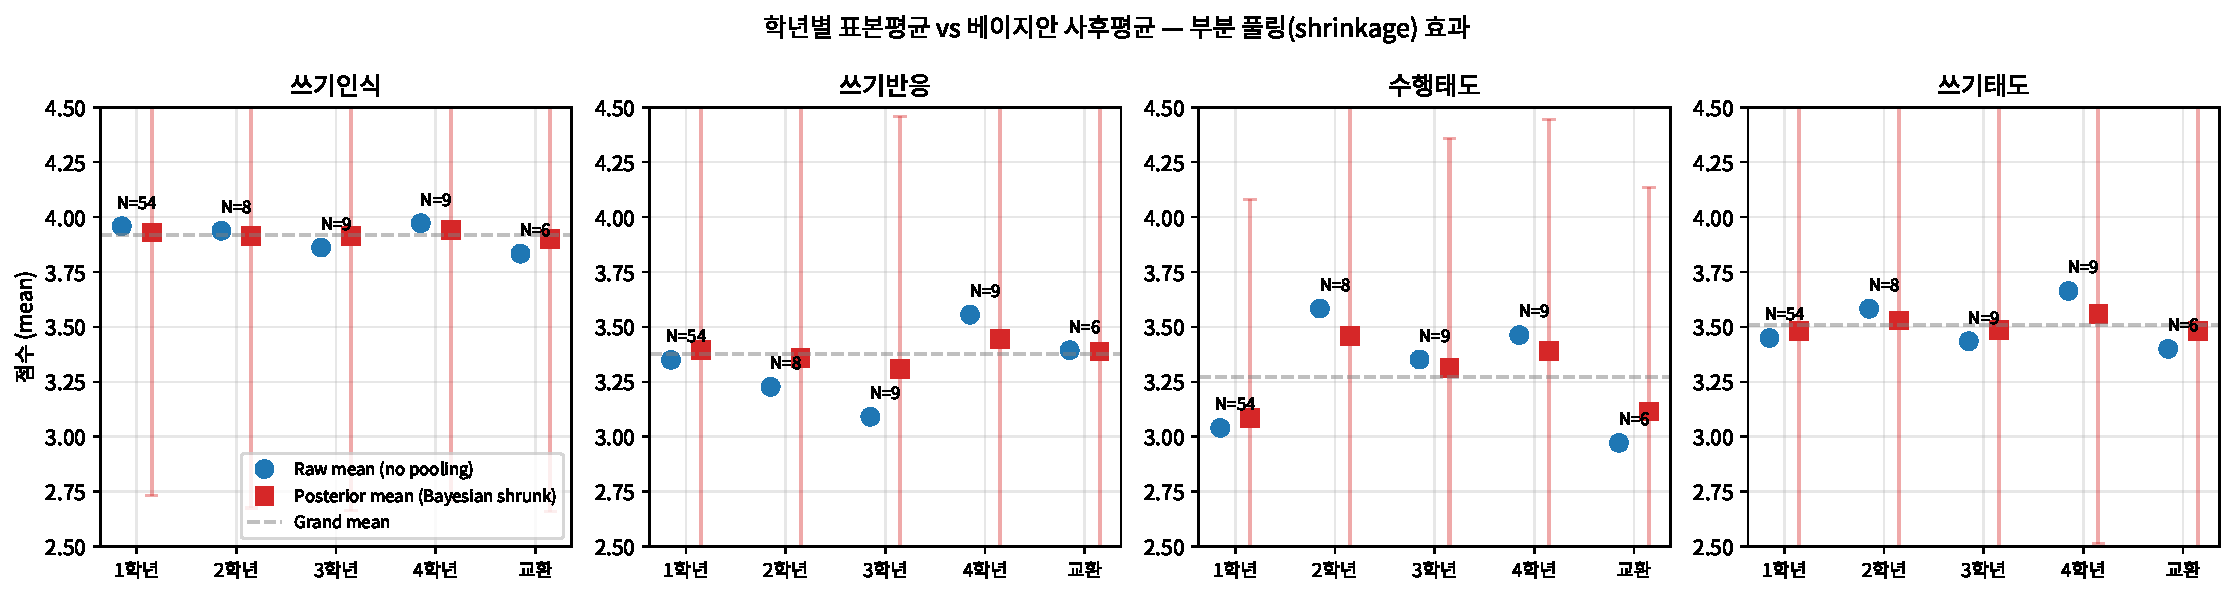
\includegraphics[width=0.95\textwidth]{gel_shrinkage_plot.pdf}

\vspace{0.3cm}
\begin{itemize}
\item 파란 원: 표본평균(raw mean) — 풀링 없음
\item 빨간 사각형: 사후평균(posterior mean) — 부분 풀링 후
\item 작은 표본 집단(2학년 $N=8$, 교환학생 $N=6$)이 전체 평균 쪽으로 \textbf{끌어당겨짐}
\end{itemize}
\end{frame}

%---------- Slide 15: Prior Distribution ----------
\begin{frame}{사전분포 선택 — 흔한 의문}
\textbf{Q}: ``효과들이 정규분포를 따른다''는 가정과 사전분포 선택이 자의적이지 않은가?

\vspace{0.3cm}
\textbf{A}: Gelman의 처방은 \textbf{약한 정보 사전분포(weakly informative prior, WIP)}:

\begin{itemize}
\item 비현실적 값만 배제, 데이터가 결정하도록 둠
\item 예: $\sigma_\alpha \sim \text{HalfNormal}(1)$ (Likert 1$-$5 척도용)
\item Inverse Gamma($\epsilon, \epsilon$) 같은 ``무정보''는 피할 것 (Gelman 2006)
\end{itemize}

\vspace{0.3cm}
\textbf{사실 빈도주의도 암묵적 사전분포를 사용:}
\begin{itemize}
\item ``평탄(flat) 사전분포''라는 \emph{매우 강한} 가정을 인식 없이 사용
\item 베이지안 WIP가 \textbf{더 명시적이고 더 합리적}
\end{itemize}

\vspace{0.2cm}
\textbf{민감도 분석(sensitivity analysis):} 여러 사전분포로 재실행 후 결론 안정성 확인.
\end{frame}

%---------- Slide 16: Code Demo ----------
\begin{frame}[fragile]{코드 한 컷 — numpyro 로 10줄}
\small
\begin{verbatim}
import numpyro, numpyro.distributions as dist
from numpyro.infer import MCMC, NUTS

def model(year_idx, y):
    mu      = numpyro.sample('mu', dist.Normal(3, 2))
    sigma_a = numpyro.sample('sigma_a', dist.HalfNormal(1.0))
    sigma_y = numpyro.sample('sigma_y', dist.HalfNormal(1.0))
    alpha   = numpyro.sample('alpha',
                  dist.Normal(0, sigma_a).expand([5]))
    numpyro.sample('y', dist.Normal(mu + alpha[year_idx], sigma_y), obs=y)

mcmc = MCMC(NUTS(model), num_warmup=500, num_samples=2000)
mcmc.run(jax.random.PRNGKey(0), year_idx=jnp.array(idx), y=jnp.array(scores))
\end{verbatim}
\normalsize

\textbf{사후표본에서 추출:}
\begin{itemize}
\item $\alpha_j - \alpha_k$: t-test 대응
\item $\sigma_\alpha$: ANOVA 대응
\item 모든 쌍별 비교: 사후비교 대응 (보정 자동)
\end{itemize}
\end{frame}

%---------- Slide 17: Frequentist vs Bayesian Comparison ----------
\begin{frame}{빈도주의 vs 베이지안 — 핵심 비교표}
\centering
\small
\begin{tabular}{lll}
\toprule
구분 & 빈도주의 & 베이지안 다층모형 \\
\midrule
2그룹 비교 & t-검정 (개별 식) & $\alpha_1 - \alpha_2$ 사후 \\
K그룹 비교 & ANOVA + 사후비교 (별도) & $\sigma_\alpha$ 사후 + 쌍별 사후 \\
다중비교 보정 & Bonferroni, FDR 등 (외부) & \textbf{부분 풀링이 자동 처리} \\
효과 크기 & 별도 계산 (Cohen's d 등) & 사후분포에서 직접 \\
불확실성 & 95\% CI (간접 해석) & 95\% 신용구간 (직접 해석) \\
작은 표본 안정성 & 불안정 (Type M 오류) & \textbf{축소(shrinkage)로 안정} \\
모형 수 & 검정마다 다른 식 & \textbf{한 식, 한 적합} \\
\bottomrule
\end{tabular}

\vspace{0.3cm}
\centering
\textbf{베이지안 다층모형은 빈도주의 검정들의 \emph{일반화(generalization)}이다.}
\end{frame}

%---------- Slide 18: Key Takeaway ----------
\begin{frame}{핵심 메시지 5가지}
\Large
\begin{enumerate}
\item \textbf{빈도주의 검정은 다층모형의 특수 경우} — 사전분포 평탄($\sigma_\alpha \to \infty$) 극한
\vspace{0.2cm}
\item \textbf{한 모형으로 모든 것} — t-test, ANOVA, 사후비교, 효과크기, 다중비교 보정 동시 처리
\vspace{0.2cm}
\item \textbf{부분 풀링이 자동 보정} — Bonferroni 불필요, 검정력 보존
\vspace{0.2cm}
\item \textbf{사전분포는 약점 아닌 명시적 도구} — 정규화(regularization)로 재해석
\vspace{0.2cm}
\item \textbf{코딩이 단순} — numpyro 10줄, lmer 1줄
\end{enumerate}
\end{frame}

%---------- Slide 19: References ----------
\begin{frame}{참고문헌 \& 추가 학습}
\textbf{핵심 논문:}
\begin{itemize}
\item Gelman, A., Hill, J., \& Yajima, M. (2012). Why We (Usually) Don't Have to Worry About Multiple Comparisons. \textit{J. Research on Educational Effectiveness}, 5, 189$-$211.
\item Gelman, A., \& Carlin, J. (2014). Beyond Power Calculations: Type S and Type M Errors. \textit{Perspectives on Psychological Science}, 9(6), 641$-$651.
\item Gelman, A. (2006). Prior distributions for variance parameters in hierarchical models. \textit{Bayesian Analysis}, 1(3), 515$-$533.
\end{itemize}

\textbf{교재:}
\begin{itemize}
\item Gelman \& Hill (2007). \textit{Data Analysis Using Regression and Multilevel/Hierarchical Models}.
\item McElreath, R. (2020). \textit{Statistical Rethinking} (2nd ed.).
\end{itemize}

\textbf{소프트웨어:}
\begin{itemize}
\item numpyro (Python), brms / rstanarm (R), Stan (다언어)
\end{itemize}
\end{frame}

%---------- Slide 20: Closing ----------
\begin{frame}
\centering
\vfill
\Huge \textbf{질문?}\\
\vspace{1cm}
\Large 다층모형으로 한 단계 더 깊은 추론을\\
\vspace{0.5cm}
\normalsize \textit{``Don't worry (much) about multiple comparisons.''}\\
$-$ Gelman, Hill \& Yajima (2012)
\vfill
\end{frame}

\end{document}
